% Options for packages loaded elsewhere
\PassOptionsToPackage{unicode}{hyperref}
\PassOptionsToPackage{hyphens}{url}
\PassOptionsToPackage{dvipsnames,svgnames,x11names}{xcolor}
%
\documentclass[
  letterpaper,
  DIV=11,
  numbers=noendperiod]{scrreprt}

\usepackage{amsmath,amssymb}
\usepackage{iftex}
\ifPDFTeX
  \usepackage[T1]{fontenc}
  \usepackage[utf8]{inputenc}
  \usepackage{textcomp} % provide euro and other symbols
\else % if luatex or xetex
  \usepackage{unicode-math}
  \defaultfontfeatures{Scale=MatchLowercase}
  \defaultfontfeatures[\rmfamily]{Ligatures=TeX,Scale=1}
\fi
\usepackage{lmodern}
\ifPDFTeX\else  
    % xetex/luatex font selection
\fi
% Use upquote if available, for straight quotes in verbatim environments
\IfFileExists{upquote.sty}{\usepackage{upquote}}{}
\IfFileExists{microtype.sty}{% use microtype if available
  \usepackage[]{microtype}
  \UseMicrotypeSet[protrusion]{basicmath} % disable protrusion for tt fonts
}{}
\makeatletter
\@ifundefined{KOMAClassName}{% if non-KOMA class
  \IfFileExists{parskip.sty}{%
    \usepackage{parskip}
  }{% else
    \setlength{\parindent}{0pt}
    \setlength{\parskip}{6pt plus 2pt minus 1pt}}
}{% if KOMA class
  \KOMAoptions{parskip=half}}
\makeatother
\usepackage{xcolor}
\setlength{\emergencystretch}{3em} % prevent overfull lines
\setcounter{secnumdepth}{5}
% Make \paragraph and \subparagraph free-standing
\makeatletter
\ifx\paragraph\undefined\else
  \let\oldparagraph\paragraph
  \renewcommand{\paragraph}{
    \@ifstar
      \xxxParagraphStar
      \xxxParagraphNoStar
  }
  \newcommand{\xxxParagraphStar}[1]{\oldparagraph*{#1}\mbox{}}
  \newcommand{\xxxParagraphNoStar}[1]{\oldparagraph{#1}\mbox{}}
\fi
\ifx\subparagraph\undefined\else
  \let\oldsubparagraph\subparagraph
  \renewcommand{\subparagraph}{
    \@ifstar
      \xxxSubParagraphStar
      \xxxSubParagraphNoStar
  }
  \newcommand{\xxxSubParagraphStar}[1]{\oldsubparagraph*{#1}\mbox{}}
  \newcommand{\xxxSubParagraphNoStar}[1]{\oldsubparagraph{#1}\mbox{}}
\fi
\makeatother

\usepackage{color}
\usepackage{fancyvrb}
\newcommand{\VerbBar}{|}
\newcommand{\VERB}{\Verb[commandchars=\\\{\}]}
\DefineVerbatimEnvironment{Highlighting}{Verbatim}{commandchars=\\\{\}}
% Add ',fontsize=\small' for more characters per line
\usepackage{framed}
\definecolor{shadecolor}{RGB}{241,243,245}
\newenvironment{Shaded}{\begin{snugshade}}{\end{snugshade}}
\newcommand{\AlertTok}[1]{\textcolor[rgb]{0.68,0.00,0.00}{#1}}
\newcommand{\AnnotationTok}[1]{\textcolor[rgb]{0.37,0.37,0.37}{#1}}
\newcommand{\AttributeTok}[1]{\textcolor[rgb]{0.40,0.45,0.13}{#1}}
\newcommand{\BaseNTok}[1]{\textcolor[rgb]{0.68,0.00,0.00}{#1}}
\newcommand{\BuiltInTok}[1]{\textcolor[rgb]{0.00,0.23,0.31}{#1}}
\newcommand{\CharTok}[1]{\textcolor[rgb]{0.13,0.47,0.30}{#1}}
\newcommand{\CommentTok}[1]{\textcolor[rgb]{0.37,0.37,0.37}{#1}}
\newcommand{\CommentVarTok}[1]{\textcolor[rgb]{0.37,0.37,0.37}{\textit{#1}}}
\newcommand{\ConstantTok}[1]{\textcolor[rgb]{0.56,0.35,0.01}{#1}}
\newcommand{\ControlFlowTok}[1]{\textcolor[rgb]{0.00,0.23,0.31}{\textbf{#1}}}
\newcommand{\DataTypeTok}[1]{\textcolor[rgb]{0.68,0.00,0.00}{#1}}
\newcommand{\DecValTok}[1]{\textcolor[rgb]{0.68,0.00,0.00}{#1}}
\newcommand{\DocumentationTok}[1]{\textcolor[rgb]{0.37,0.37,0.37}{\textit{#1}}}
\newcommand{\ErrorTok}[1]{\textcolor[rgb]{0.68,0.00,0.00}{#1}}
\newcommand{\ExtensionTok}[1]{\textcolor[rgb]{0.00,0.23,0.31}{#1}}
\newcommand{\FloatTok}[1]{\textcolor[rgb]{0.68,0.00,0.00}{#1}}
\newcommand{\FunctionTok}[1]{\textcolor[rgb]{0.28,0.35,0.67}{#1}}
\newcommand{\ImportTok}[1]{\textcolor[rgb]{0.00,0.46,0.62}{#1}}
\newcommand{\InformationTok}[1]{\textcolor[rgb]{0.37,0.37,0.37}{#1}}
\newcommand{\KeywordTok}[1]{\textcolor[rgb]{0.00,0.23,0.31}{\textbf{#1}}}
\newcommand{\NormalTok}[1]{\textcolor[rgb]{0.00,0.23,0.31}{#1}}
\newcommand{\OperatorTok}[1]{\textcolor[rgb]{0.37,0.37,0.37}{#1}}
\newcommand{\OtherTok}[1]{\textcolor[rgb]{0.00,0.23,0.31}{#1}}
\newcommand{\PreprocessorTok}[1]{\textcolor[rgb]{0.68,0.00,0.00}{#1}}
\newcommand{\RegionMarkerTok}[1]{\textcolor[rgb]{0.00,0.23,0.31}{#1}}
\newcommand{\SpecialCharTok}[1]{\textcolor[rgb]{0.37,0.37,0.37}{#1}}
\newcommand{\SpecialStringTok}[1]{\textcolor[rgb]{0.13,0.47,0.30}{#1}}
\newcommand{\StringTok}[1]{\textcolor[rgb]{0.13,0.47,0.30}{#1}}
\newcommand{\VariableTok}[1]{\textcolor[rgb]{0.07,0.07,0.07}{#1}}
\newcommand{\VerbatimStringTok}[1]{\textcolor[rgb]{0.13,0.47,0.30}{#1}}
\newcommand{\WarningTok}[1]{\textcolor[rgb]{0.37,0.37,0.37}{\textit{#1}}}

\providecommand{\tightlist}{%
  \setlength{\itemsep}{0pt}\setlength{\parskip}{0pt}}\usepackage{longtable,booktabs,array}
\usepackage{calc} % for calculating minipage widths
% Correct order of tables after \paragraph or \subparagraph
\usepackage{etoolbox}
\makeatletter
\patchcmd\longtable{\par}{\if@noskipsec\mbox{}\fi\par}{}{}
\makeatother
% Allow footnotes in longtable head/foot
\IfFileExists{footnotehyper.sty}{\usepackage{footnotehyper}}{\usepackage{footnote}}
\makesavenoteenv{longtable}
\usepackage{graphicx}
\makeatletter
\newsavebox\pandoc@box
\newcommand*\pandocbounded[1]{% scales image to fit in text height/width
  \sbox\pandoc@box{#1}%
  \Gscale@div\@tempa{\textheight}{\dimexpr\ht\pandoc@box+\dp\pandoc@box\relax}%
  \Gscale@div\@tempb{\linewidth}{\wd\pandoc@box}%
  \ifdim\@tempb\p@<\@tempa\p@\let\@tempa\@tempb\fi% select the smaller of both
  \ifdim\@tempa\p@<\p@\scalebox{\@tempa}{\usebox\pandoc@box}%
  \else\usebox{\pandoc@box}%
  \fi%
}
% Set default figure placement to htbp
\def\fps@figure{htbp}
\makeatother

\KOMAoption{captions}{tableheading}
\makeatletter
\@ifpackageloaded{bookmark}{}{\usepackage{bookmark}}
\makeatother
\makeatletter
\@ifpackageloaded{caption}{}{\usepackage{caption}}
\AtBeginDocument{%
\ifdefined\contentsname
  \renewcommand*\contentsname{Table of contents}
\else
  \newcommand\contentsname{Table of contents}
\fi
\ifdefined\listfigurename
  \renewcommand*\listfigurename{List of Figures}
\else
  \newcommand\listfigurename{List of Figures}
\fi
\ifdefined\listtablename
  \renewcommand*\listtablename{List of Tables}
\else
  \newcommand\listtablename{List of Tables}
\fi
\ifdefined\figurename
  \renewcommand*\figurename{Figure}
\else
  \newcommand\figurename{Figure}
\fi
\ifdefined\tablename
  \renewcommand*\tablename{Table}
\else
  \newcommand\tablename{Table}
\fi
}
\@ifpackageloaded{float}{}{\usepackage{float}}
\floatstyle{ruled}
\@ifundefined{c@chapter}{\newfloat{codelisting}{h}{lop}}{\newfloat{codelisting}{h}{lop}[chapter]}
\floatname{codelisting}{Listing}
\newcommand*\listoflistings{\listof{codelisting}{List of Listings}}
\usepackage{amsthm}
\theoremstyle{plain}
\newtheorem{theorem}{Theorem}[chapter]
\theoremstyle{definition}
\newtheorem{definition}{Definition}[chapter]
\theoremstyle{definition}
\newtheorem{example}{Example}[chapter]
\theoremstyle{remark}
\AtBeginDocument{\renewcommand*{\proofname}{Proof}}
\newtheorem*{remark}{Remark}
\newtheorem*{solution}{Solution}
\newtheorem{refremark}{Remark}[chapter]
\newtheorem{refsolution}{Solution}[chapter]
\makeatother
\makeatletter
\makeatother
\makeatletter
\@ifpackageloaded{caption}{}{\usepackage{caption}}
\@ifpackageloaded{subcaption}{}{\usepackage{subcaption}}
\makeatother

\usepackage{bookmark}

\IfFileExists{xurl.sty}{\usepackage{xurl}}{} % add URL line breaks if available
\urlstyle{same} % disable monospaced font for URLs
\hypersetup{
  pdftitle={MATH5835M Statistical Computing},
  pdfauthor={Matthew Aldridge},
  colorlinks=true,
  linkcolor={blue},
  filecolor={Maroon},
  citecolor={Blue},
  urlcolor={Blue},
  pdfcreator={LaTeX via pandoc}}


\title{MATH5835M Statistical Computing}
\author{Matthew Aldridge}
\date{2024-09-30}

\begin{document}
\maketitle

\renewcommand*\contentsname{Table of contents}
{
\hypersetup{linkcolor=}
\setcounter{tocdepth}{2}
\tableofcontents
}

\bookmarksetup{startatroot}

\chapter*{About MATH5835}\label{about-math5835}
\addcontentsline{toc}{chapter}{About MATH5835}

\markboth{About MATH5835}{About MATH5835}

\section*{Organisation of MATH5835}\label{organisation-of-math5835}
\addcontentsline{toc}{section}{Organisation of MATH5835}

\markright{Organisation of MATH5835}

This module is \textbf{MATH5835M Statistical Computing}.

This module lasts for 11 weeks from 29 September to 12 December 2025.
The exam will take place sometime between 12 and 23 January 2026.

The module leader, the lecturer, and the main author of these notes is
\href{https://mpaldridge.github.io/}{Dr Matthew Aldridge}. (You can call
me ``Matt'', ``Matthew'', or ``Dr Aldridge'', pronounced
``\emph{old}-ridge''.) My email address is
\href{mailto:m.aldridge@leeds.ac.uk}{\nolinkurl{m.aldridge@leeds.ac.uk}},
although I much prefer questions in person at office hours (see below)
rather than by email.

\subsection*{Lectures}\label{lectures}
\addcontentsline{toc}{subsection}{Lectures}

The main way you will learn new material for this module is by attending
lectures. There are three lectures per week:

\begin{itemize}
\item
  Mondays at 1400
\item
  Thursdays at 1200
\item
  Fridays at 1000
\end{itemize}

all in in
\href{https://students.leeds.ac.uk/buildings-and-rooms/3611/roger-stevens-lt-14-10m-14}{Roger
Stevens LT 14}.

I recommend taking your own notes during the lecture. I will put brief
summary notes from the lectures on this website, but they will not
reflect all the details I say out loud and write on the whiteboard.
Lectures will go through material quite quickly and the material may be
quite difficult, so it's likely you'll want to spend time reading
through your notes after the lecture. Lectures should be recorded on the
lecture capture system; I find it very difficult to read the whiteboard
in these videos, but if you unavoidably miss a lecture, for example due
to illness, you may find they are better than nothing.

In Weeks 3, 5, 7, 9 and 11, the Thursday lecture will operate as a
``problems class'' -- see more on this below.

Attendance at lectures in compulsory. You should record your attendance
using the UniLeeds app and the QR code on the wall in the 15 minutes
before the lecture or the 15 minutes after the lecture (but not during
the lecture).

\subsection*{Problem sheets and problem
classes}\label{problem-sheets-and-problem-classes}
\addcontentsline{toc}{subsection}{Problem sheets and problem classes}

Mathematics and statistics are ``doing'' subjects! To help you learn
material for the module and to help you prepare for the exam, I will
provide 5 unassessed problem sheets. These are for you to work through
in your own time to help you learn; they are \emph{not} formally
assessed. You are welcome to discuss work on the problem sheets with
colleagues and friends, although my recommendation would be to write-up
your ``last, best'' attempt neatly by yourself.

There will be an optional opportunity to submit one or two questions
from the problem sheet to me in advance of the problems class for some
brief informal feedback on your work. See the problem sheets for
details.

You should work through each problem sheet in preparation for the
problems class in the Thursday lecture of Week 3, 5, 7, 9 and 11. In the
problems class, you should be ready to explain your answers to questions
you managed to solve, discuss your progress on questions you partially
solved, and ask for help on questions you got stuck on.

You can also ask for extra help or feedback at office hours (see below).

\subsection*{Coursework}\label{coursework}
\addcontentsline{toc}{subsection}{Coursework}

There will be one piece of assessed coursework, which will make up 20\%
of your module mark. \hyperref[coursework]{You can read more about the
coursework here.}

The coursework will be in the form of a worksheet. The worksheet will
have some questions, mostly computational but also mathematical, and you
will have to write a report containing your answers and computations.

The assessed coursework will be introduced in the \textbf{computer
practical} sessions in Week 9.

The deadline for the coursework will be the penultimate day of the
Autumn term, \textbf{Thursday 12 December } at 1400. Feedback and marks
will be returned on Monday 13 January, the first day of the Spring term.

\subsection*{Office hours}\label{office-hours}
\addcontentsline{toc}{subsection}{Office hours}

I will run a n optional ``office hours'' drop-in session each week for
feedback and consultation. You can come along if you want to talk to me
about anything on the module, including if you'd like more feedback on
your attempts at problem sheet questions. (For extremely short queries,
you can approach me before or after lectures, but my response will often
be: ``Come to my office hours, and we can discuss it there!'')

Office hours will happen on \textbf{Thursdays from 1300 to 1400} -- so
directly after the Thursday lecture / problems class -- in my office,
which is \textbf{EC Stoner 9.10n} in ``Maths Research Deck'' area on the
9th floor of the EC Stoner building. (One way to the Maths Research Deck
is via the doors directly opposite the main entrance to the School of
Mathematics; you can also get there from Staircase 1 on the Level 10
``red route'' through EC Stoner, next to the Maths Satellite.) If you
cannot make this time, contact me for an alternative arrangement.

\subsection*{Exam}\label{exam}
\addcontentsline{toc}{subsection}{Exam}

There will be one exam, which will make up 80\% of your module mark.

The exam will be in the January 2026 exam period (12--23 January); the
date and time will be announced in December. The exam will be in person
and on campus.

The exam will last 2 hours and 30 minutes. The exam will consist of 4
questions, all compulsory. You will be allowed to use a permitted
calculator in the exam.

\section*{Content of MATH5835}\label{content-of-math5835}
\addcontentsline{toc}{section}{Content of MATH5835}

\markright{Content of MATH5835}

\subsection*{Necessary background}\label{necessary-background}
\addcontentsline{toc}{subsection}{Necessary background}

I recommend that students should have completed at least two
undergraduate level courses in probability or statistics -- although
confidence and proficiency in basic material is more important than very
deep knowledge of more complicated topics.

For Leeds undergraduates, MATH2715 Statistical Methods is an official
prerequisite (please get in touch with me if you are/were a Leeds
undergraduate and have not taken MATH2715), although confidence and
proficiency in the more basic material of MATH1710 \& MATH1712
Probability and Statistics 1 \& 2 is probably more important.

Some knowledge I will assume:

\begin{itemize}
\item
  \textbf{Probability:} Basic rules of probability; random variables,
  both continuous and discrete; ``famous'' distributions (especially the
  normal distribution and the continuous uniform distribution);
  expectation, variance, covariance, correlation; law of large numbers
  and central limit theorem.
\item
  \textbf{Statistics:} Estimation of parameters; bias and error; sample
  mean and sample variance
\end{itemize}

This module will also include an material on Markov chains. I won't
assume any pre-existing knowledge of this, and I will introduce all new
material we need, but students who have studied Markov chains before
(for example in the Leeds module MATH2750 Introduction to Markov
Processes) may find a couple of lectures here are merely a reminder of
things they already know.

The lectures will include examples using the \textbf{R} program
language. The coursework and problem sheets will require use of R. The
exam, while just a ``pencil and paper'' exam, will require understanding
and writing short portions of R code. We will assume basic R capability
-- that you can enter R commands, store R objects using the
\texttt{\textless{}-} assignment, and perform basic arithmetic with
numbers and vectors. Other concepts will be introduced as necessary. If
you want to use R on your own device, I recommend downloading (if you
have not already) the \href{https://cran.r-project.org}{R programming
language} and the \href{https://posit.co/downloads/}{program RStudio}.
(These lecture notes were written in R using RStudio.)

\subsection*{Syllabus}\label{syllabus}
\addcontentsline{toc}{subsection}{Syllabus}

We plan to cover the following topics in the module:

\begin{itemize}
\item
  \textbf{Monte Carlo estimation:} definition and examples; bias and
  error; variance reduction techniques: control variates, antithetic
  variables, importance sampling. {[}9 lectures{]}
\item
  \textbf{Random number generation:} pseudo-random number generation
  using linear congruential generators; inverse transform method;
  rejection sampling {[}7 lectures{]}
\item
  \textbf{Markov chain Monte Carlo} (MCMC)\textbf{:} {[}7 lectures{]}

  \begin{itemize}
  \item
    Introduction to Markov chains in discrete and continuous space
  \item
    Metropolis--Hastings algorithm: definition; examples; MCMC in
    practice; MCMC for Bayesian statistics
  \end{itemize}
\item
  \textbf{Resampling methods:} Empirical distribution; plug-in
  estimation; bootstrap statistics; bootstrap estimation {[}4
  lectures{]}
\item
  Frequently-asked questions {[}1 lecture{]}
\end{itemize}

Together with the 5 problems classes, this makes 33 lectures.

\subsection*{Book}\label{book}
\addcontentsline{toc}{subsection}{Book}

The following book is strongly recommended for the module:

\begin{itemize}
\tightlist
\item
  J Voss,
  \href{https://leeds.primo.exlibrisgroup.com/permalink/44LEE_INST/1fj430b/cdi_askewsholts_vlebooks_9781118728031}{\emph{An
  Introduction to Statistical Computing: A simulation-based approach}},
  Wiley Series in Computational Statistics, Wiley, 2014
\end{itemize}

The library has
\href{https://leeds.primo.exlibrisgroup.com/permalink/44LEE_INST/1fj430b/cdi_askewsholts_vlebooks_9781118728031}{electronic
access to this book} (and two paper copies).

Dr Voss is a lecturer in the School of Mathematics and the University of
Leeds, and has taught MATH5835 many times. \emph{An Introduction to
Statistical Computing} grew out of his lecture notes for this module, so
the book is ideally suited for this module. My lectures will follow this
book closely -- specifically:

\begin{itemize}
\item
  Monte Carlo estimation: Sections 3.1--3.3
\item
  Random number generation: Sections 1.1--1.4
\item
  Markov chain Monte Carlo: Section 2.3 and Sections 4.1--4.3
\item
  Bootstrap: Section 5.2
\end{itemize}

For a second look at material, for preparatory reading, for optional
extended reading, or for extra exercises, this book comes with my
highest recommendation!

\part{Monte Carlo estimation}

\chapter{Introduction to Monte Carlo}\label{introduction-to-monte-carlo}

\[\newcommand{\Exg}{\operatorname{\mathbb{E}}} 
\newcommand{\Ex}{\mathbb{E}} 
\newcommand{\Ind}{\mathbb{I}}
\newcommand{\Var}{\operatorname{Var}}
\newcommand{\Cov}{\operatorname{Cov}}
\newcommand{\Corr}{\operatorname{Corr}}
\newcommand{\ee}{\mathrm{e}}\]

Today, we'll start the first main topic of the module, which is called
``Monte Carlo estimation''. But first, a bit about the subject as a
whole.

\section{What is statistical
computing?}\label{what-is-statistical-computing}

``Statistical computing'' -- or ``computational statistics'' -- refers
to the branch of statistics that involves not attacking statistical
problems merely with a pencil and paper, but rather by combining human
ingenuity with the immense calculating powers of computers.

One of the big ideas here is \textbf{simulation}. Simulation is the idea
that we can understand the properties of a random model not by cleverly
working out the properties using theory -- this is usually impossible
for anything but the simplest ``toy models'' -- but rather by running
the model many times on a computer. From these many simulations, we can
observe and measure things like the typical (or ``expected'') behaviour,
the spread (or ``variance'') of the behaviour, and other things. This
concept of simulation is at the heart of the module MATH5835M
Statistical Computing.

In particular, we will look at \textbf{Monte Carlo} estimation. Monte
Carlo is about estimating a parameter, expectation or probability
related to a random variable by taking many samples of that random
variable, then computing a relevant sample mean from those samples. We
will study Monte Carlo in its standard ``basic'' form, then look at ways
we can make Monte Carlo estimation more accurate (Lectures 1--9).

To run a simulation -- for example, when performing Monte Carlo
estimation -- one needs random numbers with the correct distribution.
\textbf{Random number generation} (Lectures 10--16) will be an important
part of this module. We will look first at how to generate randomness of
any sort, and then how to manipulate that randomness into the shape of
the distributions we want.

Sometimes, it's not possible to generate perfectly independent samples
from exactly the distribution you want. But we can use the output of a
process called a ``Markov chain'' to get ``fairly independent'' samples
from nearly the distribution we want. When we perform Monte Carlo
estimation with the output of a Markov chain, this is called
\textbf{Markov chain Monte Carlo (MCMC)} (Lectures 17--23). MCMC has
become a vital part of modern Bayesian statistical analysis.

The final section of the module is about dealing with data. Choosing a
random piece of data from a given dataset is a lot like generating a
random number from a given distribution, and similar Monte Carlo
estimation ideas can be used to find out about that data. We think of a
dataset as being a sample from a population, and sampling again from
that dataset is known as \textbf{resampling} (Lecture 24--27). The most
important method of finding out about a population by using resampling
from a dataset is called the ``bootstrap'', and we will study the
bootstrap in detail.

MATH5835M Statistical Computing is a \emph{mathematics} module that will
concentrate on the \emph{mathematical} ideas that underpin statistical
computing. It is not a programming module that will go deeply into the
practical issues of the most efficient possible coding of the algorithms
we study. But we will want to investigate the behaviour of the methods
we learn about and to explore their properties, so will be computer
programming to help us do that. We will be using the statistical
programming language R, (although one could just as easily have used
Python or other similar languages). As my PhD supervisor often told me:
``You don't really understand a mathematical algorithm until you've
coded it up yourself.''

\section{What is Monte Carlo
estimation?}\label{what-is-monte-carlo-estimation}

Let \(X\) be a random variable. We recall the \textbf{expectation}
\(\Ex X\) of \(X\). If \(X\) is discrete with probability mass function
(PMF) \(p\), then the expectation of \(X\) is
\[ \Ex X = \sum_x x\,p(x) ;\] while if \(X\) is continuous with
probability density function (PDF) \(f\), then the expectation is
\[ \Ex X = \int_{-\infty}^{+\infty} x\,f(x)\,\mathrm{d}x . \] More
generally, the expectation of a function \(\phi\) of \(X\) is
\[ \Exg \phi(X) = \begin{cases} {\displaystyle \sum_x \phi(x)\,p(x)} & \text{for $X$ discrete}\\ {\displaystyle \int_{-\infty}^{+\infty} \phi(x)\,f(x)\,\mathrm{d}x}  & \text{for $X$ continuous.} \end{cases}\]
(This matches with the ``plain'' expectation when \(\phi(x) = x\).)

But how do we actually \emph{calculate} an expectation like one of
these? If \(X\) is discrete and can only take a small, finite number of
values, then we can simply add up the sum \(\sum_x \phi(x)\,p(x)\). But
otherwise, we just have to hope that \(\phi\) and \(p\) or \(f\) are
sufficiently ``nice'' that we can manage to work out the sum/integral
using a pencil and paper (and our brain). But while this is often
possible in the sort of ``toy example'' one comes across in maths or
statistics lectures, this is very rare in ``real life'' problems.

\textbf{Monte Carlo estimation} is the idea that we can get an
approximate answer for \(\Ex X\) or \(\Exg \phi(X)\) if we have access
to lots of samples from \(X\). If we have access to
\(X_1, X_2 \dots, X_n\) , independent and identically distributed (IID)
samples with the same distribution as \(X\), then we already know that
the mean
\[ \overline X = \frac{1}{n}(X_1 + X_2 + \cdots + X_n) = \frac{1}{n} \sum_{i=1}^n X_i \]
can be used to estimate the expectation \(\mathbb EX\). We know that
\(\overline X\) is usually close to the expectation \(\Ex X\), at least
if if the number of samples \(n\) is large; this is justified by the
``law of large numbers'', which says that \(\overline X \to \mathbb EX\)
as \(n \to \infty\).

Similarly, we can use
\[ \frac{1}{n} \big(\phi(X_1) + \phi(X_2) + \cdots + \phi(X_n) \big) = \frac{1}{n} \sum_{i=1}^n \phi(X_i) \]
to estimate \(\Exg \phi(X)\). The law of large numbers again says that
this estimate tends to the correct value \(\Exg \phi(X)\) as
\(n \to \infty\).

In this module we will write that \(X_1, X_2, \dots, X_n\) is a
``\textbf{random sample} from \(X\)'' to mean that
\(X_1, X_2, \dots, X_n\) are IID with the same distribution as \(X\).

\begin{definition}[]\protect\hypertarget{def-MCest}{}\label{def-MCest}

Let \(X\) be a random variable, \(\phi\) a function, and write
\(\theta = \Exg\phi(X)\). Then the \textbf{Monte Carlo estimator}
\(\widehat\theta_n^{\mathrm{MC}}\) of \(\theta\) is
\[ \widehat{\theta}_n^{\mathrm{MC}} = \frac{1}{n} \sum_{i=1}^n \phi(X_i) , \]
where \(X_1, X_2, \dots, X_n\) are a random sample from \(X\).

\end{definition}

While general ideas for estimating using simulation go back a long time,
the modern theory of Monte Carlo estimation was developed by the
physicists \href{https://en.wikipedia.org/wiki/Stanisław_Ulam}{Stanislaw
Ulam} and \href{https://en.wikipedia.org/wiki/John_von_Neumann}{John von
Neumann}. Ulam (who was Polish) and von Neumann (who was Hungarian)
moved to the US in the early 1940s to work on the Manhattan project to
build the atomic bomb (as made famous by the film \emph{Oppenheimer}).
Later in the 1940s, they worked together in the Los Alamos National
Laboratory continuing their research on nuclear physics generally and
nuclear weapons more specifically, where they used simulations on early
computers to help them numerically solve difficult mathematical and
physical problems.

The name ``Monte Carlo'' was chosen because the use of randomness to
solve such problems reminded them of gamblers in the casinos of Monte
Carlo, Monaco. Ulam and von Neumann also worked closely with another
colleague Nicholas Metropolis, whose work we will study later in this
module.

\section{Examples}\label{examples}

Let's see some simple examples of Monte Carlo estimation using R.

\begin{example}[]\protect\hypertarget{exm-MCexp}{}\label{exm-MCexp}

Let's suppose we've forgotten the expectation of the exponential
distribution \(X \sim \operatorname{Exp}(2)\) with rate 2. In this
simple case, we could work out the answer using the PDF
\(f(x) = 2\mathrm{e}^{-2x}\) as\\
\[ \mathbb E X = \int_0^\infty x\,2\mathrm{e}^{-2x}\,\mathrm{d}x \]and,
without too much difficulty, get the answer \(\frac12\). But instead,
let's do this the Monte Carlo way.

In R, we can use the \texttt{rexp()} function to get IID samples from
the exponential distribution: the full syntax is
\texttt{rexp(n,\ rate)}, which gives \texttt{n} samples from an
exponential distribution with rate \texttt{rate}. The following code
takes the mean of \(n = 100\) samples from the exponential distribution.

\begin{Shaded}
\begin{Highlighting}[]
\NormalTok{n }\OtherTok{\textless{}{-}} \DecValTok{100}
\NormalTok{samples }\OtherTok{\textless{}{-}} \FunctionTok{rexp}\NormalTok{(n, }\DecValTok{2}\NormalTok{)}
\NormalTok{MCest }\OtherTok{\textless{}{-}}\NormalTok{ (}\DecValTok{1} \SpecialCharTok{/}\NormalTok{ n) }\SpecialCharTok{*} \FunctionTok{sum}\NormalTok{(samples)}
\NormalTok{MCest}
\end{Highlighting}
\end{Shaded}

\begin{verbatim}
[1] 0.4594331
\end{verbatim}

So our Monte Carlo estimate is 0.4594, to 4 decimal places.

That's fairly close to the correct answer of \(\frac12\). But we should
(hopefully) be able to get a more accurate estimation if we use more
samples. We could also simplify the third line of our code by using the
\texttt{mean()} function.

\begin{Shaded}
\begin{Highlighting}[]
\NormalTok{n }\OtherTok{\textless{}{-}} \FloatTok{1e6}
\NormalTok{samples }\OtherTok{\textless{}{-}} \FunctionTok{rexp}\NormalTok{(n, }\DecValTok{2}\NormalTok{)}
\NormalTok{MCest }\OtherTok{\textless{}{-}} \FunctionTok{mean}\NormalTok{(samples)}
\NormalTok{MCest}
\end{Highlighting}
\end{Shaded}

\begin{verbatim}
[1] 0.4996347
\end{verbatim}

In the second line, \texttt{1e6} is R code for the scientific notation
\(1 \times 10^6\), or a million. I just picked this as ``a big number,
but where my code still only took a few seconds to run.''

Our new Monte Carlo estimate is 0.4996, which is (probably) much closer
to the true value of \(\frac12\).

\end{example}

By the way: all R code ``chunks'' displayed in the notes should work
perfectly if you copy-and-paste them into RStudio. (Indeed, when I
compile these lecture notes in RStudio, all the R code gets run on my
computer -- so I'm certain in must work correctly!) If you hover over a
code chunk, a little ``clipboard'' icon should appear in the top-right,
and clicking on that will copy it so you can paste it into RStudio. I
strongly encourage playing about with the code as a good way to learn
this material and explore further!

\begin{example}[]\protect\hypertarget{exm-MC2}{}\label{exm-MC2}

Let's try another example. Let \(X \sim \operatorname{N}(1, 2^2)\) be a
normal distribution with mean 1 and standard deviation 2. Suppose we
want to find out \(\mathbb E(\sin X)\) (for some reason). While it
\emph{might} be possible to somehow calculate the integral
\[ \mathbb E(\sin X) = \int_{-\infty}^{+\infty} (\sin x) \, \frac{1}{\sqrt{2\pi\times 2^2}} \exp\left(-\frac{(x - 1)^2}{2\times 2^2}\right) \, \mathrm{d} x , \]
that looks extremely difficult to me.

Instead, a Monte Carlo estimation of \(\mathbb{E}(\sin X)\) is very
straightforward: we just take the mean of the sine of a bunch of
normally distributed random numbers. That is we get a random samples
\(X_1, X_2, \dots, X_n\) from \(X\); then take the mean of the values
\[\sin(X_1), \sin(X_2), \dots, \sin(X_n) .\]

(We must remember, though, when using the \texttt{rnorm()} function to
generate normally distributed random variates, that the third argument
is the \emph{standard deviation}, here \(2\), \emph{not} the variance,
here \(2^2 = 4\).)

\begin{Shaded}
\begin{Highlighting}[]
\NormalTok{n }\OtherTok{\textless{}{-}} \FloatTok{1e6}
\NormalTok{samples }\OtherTok{\textless{}{-}} \FunctionTok{rnorm}\NormalTok{(n, }\DecValTok{1}\NormalTok{, }\DecValTok{2}\NormalTok{)}
\NormalTok{MCest }\OtherTok{\textless{}{-}} \FunctionTok{mean}\NormalTok{(}\FunctionTok{sin}\NormalTok{(samples))}
\NormalTok{MCest}
\end{Highlighting}
\end{Shaded}

\begin{verbatim}
[1] 0.1131249
\end{verbatim}

Our Monte Carlo estimate is 0.11312.

\end{example}

\textbf{Next time:} \emph{We look at more examples of things we can
estimate using the Monte Carlo method.}

\textbf{Summary:}

\begin{itemize}
\item
  Statistical computing is about solving statistical problems by
  combining human ingenuity with computing power.
\item
  The Monte Carlo estimate of \(\Exg \phi(X)\) is
  \[ \widehat{\theta}_n^{\mathrm{MC}} = \frac{1}{n} \sum_{i=1}^n \phi(X_i) , \]
  where \(X_1, \dots, X_n\) are IID random samples from \(X\).
\item
  Monte Carlo estimation typically gets more accurate as the number of
  samples \(n\) gets bigger.
\end{itemize}

\textbf{Read more:}
\href{https://leeds.primo.exlibrisgroup.com/permalink/44LEE_INST/1fj430b/cdi_askewsholts_vlebooks_9781118728031}{Voss,
\emph{An Introduction to Statistical Computing}}, Section 3.1 and
Subsection 3.2.1.

\chapter{Uses of Monte Carlo}\label{uses-of-monte-carlo}

\[\newcommand{\Exg}{\operatorname{\mathbb{E}}} 
\newcommand{\Ex}{\mathbb{E}} 
\newcommand{\Ind}{\mathbb{I}}
\newcommand{\Var}{\operatorname{Var}}
\newcommand{\Cov}{\operatorname{Cov}}
\newcommand{\Corr}{\operatorname{Corr}}
\newcommand{\ee}{\mathrm{e}}\]

Quick recap: Last time we defined the Monte Carlo estimator for an
expectation of a function of a random variable \(\theta = \Exg \phi(X)\)
to be
\[ \widehat{\theta}_n^{\mathrm{MC}} = \frac{1}{n} \big(\phi(X_1) + \phi(X_2) + \cdots + \phi(X_n) \big) = \frac{1}{n} \sum_{i=1}^n \phi(X_i) , \]
where \(X_1, X_2, \dots, X_n\) are independent random samples from
\(X\).

Today we look at two other things we can estimate using Monte Carlo
simulation: probabilities, and integrals.

\section{Monte Carlo for
probabilities}\label{monte-carlo-for-probabilities}

What if we want to find a \emph{probability}, rather than an
expectation? What if we want \(\mathbb P(X = x)\) for some \(x\), or
\(\mathbb P(X \geq a)\) for some \(a\), or, more generally,
\(\mathbb P(X \in A)\) for some set \(A\)?

The key thing that will help us here is the \emph{indicator function}.
The indicator function simply tells us whether an outcome \(x\) is in a
set \(A\) or not.

\begin{definition}[]\protect\hypertarget{def-indicator}{}\label{def-indicator}

Let \(A\) be a set. Then the \textbf{indicator function} \(\Ind_A\) is
defined by
\[ \Ind_A(x) = \begin{cases} 1 & \text{if $x \in A$} \\ 0 & \text{if $x \notin A$.} \end{cases} \]

\end{definition}

The set \(A\) could just be a single element \(A = \{y\}\). In that case
\(\Ind_A(x)\) is 1 if \(x = y\) and 0 if \(x \neq y\). Or \(A\) could be
a semi-infinite interval, like \(A = [a, \infty)\). In that case
\(\Ind_A(x)\) is 1 if \(x \geq a\) and 0 if \(x < a\).

Why is this helpful? Well \(\Ind_A\) is a function, so let's think about
what the expectation \(\Exg \Ind_A(X)\) would be for some random
variable \(X\). Since \(\Ind_A\) can only take two values, 0 and 1, we
have \[ \begin{align*}
\Exg \Ind_A(X) &= \sum_{y \in\{0,1\}} y\,\mathbb P\big( \Ind_A(X) = y \big) \\\
  &= 0 \times \mathbb P\big( \Ind_A(X) = 0 \big) + 1 \times \mathbb P\big( \Ind_A(X) = 1 \big) \\
  &= 0 \times \mathbb P(X \notin A) + 1 \times \mathbb P(X \in A) \\
  &= \mathbb P(X \in A) .
\end{align*} \] In line three, we used that \(\Ind_A(X) = 0\) if and
only if \(X \notin A\), and that \(\Ind_A(X) = 1\) if and only if
\(X \in A\).

So the expectation of an indicator function a set is the probability
that \(X\) is in that set. This idea connects ``expectations of
functions'' back to probabilities: if we want to find
\(\mathbb P(X \in A)\) we can find the expectation of \(\Ind_A(X)\).

With this idea in hand, how do we estimate
\(\theta = \mathbb P(X \in A)\) using the Monte Carlo method? We write
\(\theta = \Exg\Ind_A(X)\). Then our Monte Carlo estimator is
\[  \widehat{\theta}_n^{\mathrm{MC}} = \frac{1}{n} \sum_{i=1}^n \Ind_A(X_i) . \]

We remember that \(\Ind_A(X_i)\) is 1 if \(X_i \in A\) and 0 otherwise.
So if we add up \(n\) of these, we count an extra +1 each time we have
an \(X_i \in A\). So \(\sum_{i=1}^n \Ind_A(X_i)\) counts the total
number of the \(X_i\) that are in \(A\). So the Monte Carlo estimator
can be written as
\[  \widehat{\theta}_n^{\mathrm{MC}} = \frac{\# \text{ of } X_i \text{ that are in $A$}}{n} . \]
(I'm using \(\#\) as shorthand for ``the number of''.)

Although we've had to do a bit of work to get here, this a totally
logical outcome! The right-hand side here is the proportion of the
samples for which \(X_i \in A\). And if we want to estimate the
probability something happens, looking at the proportion of times it
happens in a random sample is very much the ``intuitive'' estimate to
take. And that intuitive estimate is indeed the Monte Carlo estimate!

\begin{example}[]\protect\hypertarget{exm-MCprob}{}\label{exm-MCprob}

\emph{Let} \(Z \sim \operatorname{N}(0,1)\) \emph{be a standard normal
distribution. Estimate} \(\mathbb P(Z > 2)\)\emph{.}

This is a question that it is impossible to answer exactly using a
pencil and paper: there's no closed form for
\[ \mathbb P(Z > 2) = \int_2^\infty \frac{1}{\sqrt{2\pi}}\,\mathrm{e}^{-z^2/2}\,\mathrm{d}z , \]
so we'll have to use an estimation method.

The Monte Carlo estimate means taking a random sample
\(Z_1, Z_2, \dots, Z_n\) of standard normals, and calculating what
proportion of them are greater than 2. In R, we can do this as follows.

\begin{Shaded}
\begin{Highlighting}[]
\NormalTok{n }\OtherTok{\textless{}{-}} \FloatTok{1e6}
\NormalTok{samples }\OtherTok{\textless{}{-}} \FunctionTok{rnorm}\NormalTok{(n)}
\NormalTok{MCest }\OtherTok{\textless{}{-}} \FunctionTok{mean}\NormalTok{(samples }\SpecialCharTok{\textgreater{}} \DecValTok{2}\NormalTok{)}
\NormalTok{MCest}
\end{Highlighting}
\end{Shaded}

\begin{verbatim}
[1] 0.022716
\end{verbatim}

In the second line, we could have written \texttt{rnorm(n,\ 0,\ 1)}.
But, if you don't give the parameters \texttt{mean} and \texttt{sd} to
the function \texttt{rnorm()}, R just assumes you want the standard
normal with \texttt{mean\ =\ 0} and \texttt{sd\ =\ 1}.

We can check our answer: R's inbuilt \texttt{pnorm()} function estimates
probabilities for the normal distribution (using a method that, in this
specific case, is much quicker and more accurate than Monte Carlo
estimation). The true answer is very close to

\begin{Shaded}
\begin{Highlighting}[]
\FunctionTok{pnorm}\NormalTok{(}\DecValTok{2}\NormalTok{, }\AttributeTok{lower.tail =} \ConstantTok{FALSE}\NormalTok{)}
\end{Highlighting}
\end{Shaded}

\begin{verbatim}
[1] 0.02275013
\end{verbatim}

so our estimate was pretty good.

\end{example}

We should explain the third line in the code we used for the Monte Carlo
estimation \texttt{mean(samples\ \textgreater{}\ 2)}. In R, some
statements can be answered ``true'' or ``false'': these are often
statements involving equality \texttt{==} (that's a \emph{double} equals
sign) or inequalities like \texttt{\textless{}}, \texttt{\textless{}=},
\texttt{\textgreater{}=}, \texttt{\textgreater{}}, for example. So
\texttt{5\ \textgreater{}\ 2} is \texttt{TRUE} but \texttt{3\ ==\ 7} is
\texttt{FALSE}. These can be applied ``component by component'' to
vectors. So, for example, testing which numbers from 1 to 10 are greater
than or equal to 7, we get

\begin{Shaded}
\begin{Highlighting}[]
\DecValTok{1}\SpecialCharTok{:}\DecValTok{10} \SpecialCharTok{\textgreater{}=} \DecValTok{7}
\end{Highlighting}
\end{Shaded}

\begin{verbatim}
 [1] FALSE FALSE FALSE FALSE FALSE FALSE  TRUE  TRUE  TRUE  TRUE
\end{verbatim}

six \texttt{FALSE}s (for 1 to 6) followed by four \texttt{TRUE}s (for 7
to 10).

We can also use \texttt{\&} (``and'') and \texttt{\textbar{}} (``or'')
in true/false statements like these.

But R also knows to treat \texttt{TRUE} like the number 1 and
\texttt{FALSE} like the number 0. (This is just like the concept of the
indicator function we've been discussing.) So if we add up some
\texttt{TRUE}s and \texttt{FALSE}s, R simply counts how many
\texttt{TRUE}s there are

\begin{Shaded}
\begin{Highlighting}[]
\FunctionTok{sum}\NormalTok{(}\DecValTok{1}\SpecialCharTok{:}\DecValTok{10} \SpecialCharTok{\textgreater{}=} \DecValTok{7}\NormalTok{)}
\end{Highlighting}
\end{Shaded}

\begin{verbatim}
[1] 4
\end{verbatim}

So in our Monte Carlo estimation code,
\texttt{samples\ \textgreater{}\ 2} was a vector of \texttt{TRUE}s and
\texttt{FALSE}s, depending on whether each sample was greater than 2 or
not, then \texttt{mean(samples\ \textgreater{}\ 2)} took the
\emph{proportion} of the samples that were greater than 2.

\section{Monte Carlo for integrals}\label{monte-carlo-for-integrals}

There's another thing -- a non-statistics thing -- that Monte Carlo
estimation is useful for. We can use Monte Carlo estimation to
approximate integrals that are too hard to do by hand.

This might seem surprising. Estimating the expectation of (a function
of) a random variable seems a naturally statistical thing to do. But an
integral is just a straight maths problem -- there's not any randomness
at all. But actually, integrals and expectations are very similar
things.

Let's think of an integral: say, \[ \int_a^b h(x) \,\mathrm{d}x ,\] the
integral of some function \(h\) (the ``integrand'') between the limits
\(a\) and \(b\). Now let's compare that to the integral \(\Exg \phi(X)\)
of a continuous random variable that we can estimate using Monte Carlo
estimation,
\[ \Exg \phi(X) = \int_{-\infty}^\infty \phi(x)\,f(x)\, \mathrm{d} x. \]
Matching things up, we can see that we if we were to a function \(\phi\)
and a PDF \(f\) such that
\begin{equation}\phantomsection\label{eq-match}{ \phi(x)\,f(x) = \begin{cases} 0 & x < a \\ h(x) & a \leq x \leq b \\ 0 & x > b , \end{cases} }\end{equation}
then we would have
\[ \Exg \phi(X) = \int_{-\infty}^\infty \phi(x)\,f(x)\, \mathrm{d} x = \int_a^b h(x) \,\mathrm{d}x, \]
so the value of the expectation would be precisely the value of the
integral we're after. Then we could use Monte Carlo to estimate that
expectation/integral.

There are lots of choices of \(\phi\) and \(f\) that would satisfy this
the condition in Equation~\ref{eq-match}. But a ``common-sense'' choice
that often works is to pick \(f\) to be the PDF of \(X\), a continuous
uniform distribution on the interval \([a,b]\). (This certainly works
when \(a\) and \(b\) are finite, anyway.) Recall that the continuous
uniform distribution means that \(X\) has PDF
\[ f(x) = \begin{cases} 0 & x < a \\ \displaystyle{\frac{1}{b-a}} & a \leq x \leq b \\ 0 & x > b . \end{cases} \]
Comparing this equation with Equation~\ref{eq-match}, we then have to
choose \[\phi(x) = \frac{h(x)}{f(x)} = (b-a)h(x).\]

Putting this all together, we have
\[ \Exg \phi(X) = \int_{-\infty}^{+\infty} \phi(x)\,f(x)\,\mathrm{d}x = \int_a^b (b-a)h(x)\,\frac{1}{b-a}\,\mathrm{d}x = \int_a^b h(x) \,\mathrm{d}x ,\]
as required. This can then be estimated using the Monte Carlo method.

\begin{definition}[]\protect\hypertarget{def-MCint}{}\label{def-MCint}

Consider an integral \(\theta = \int_a^b h(x)\,\mathrm{d}x\). Let \(f\)
be the probability density function of a random variable \(X\) and let
\(\phi\) be function such that Equation~\ref{eq-match} holds. Then the
\textbf{Monte Carlo estimator} \(\widehat\theta_n^{\mathrm{MC}}\) of the
integral \(\theta\) is
\[ \widehat{\theta}_n^{\mathrm{MC}} = \frac{1}{n} \sum_{i=1}^n \phi(X_i) , \]
where \(X_1, X_2, \dots, X_n\) are a random sample from \(X\).

\end{definition}

\begin{example}[]\protect\hypertarget{exm-MCint}{}\label{exm-MCint}

Suppose we want to approximate the integral
\[ \int_0^2 x^{1.6} (2-x)^{0.7} \, \mathrm{d}x . \]

Since this is an integral on the finite interval \([0,2]\), it would
seem to make sense to pick \(X\) to be uniform on \([0,2]\). This means
we should take
\[\phi(x) = \frac{h(x)}{f(x)} = (2-0)h(x) = 2\,x^{1.6}(2-x)^{0.7}.\] We
can then approximate this integral in R using the Monte Carlo estimator
\[ \int_0^2 x^{1.6} (2-x)^{0.7} \, \mathrm{d}x = \operatorname{\mathbb{E}} \phi(X) \approx \frac{1}{n} \sum_{i=1}^n 2\,X_i^{1.6} (2-X_i)^{0.7} . \]

\begin{Shaded}
\begin{Highlighting}[]
\NormalTok{n }\OtherTok{\textless{}{-}} \FloatTok{1e6}
\NormalTok{integrand }\OtherTok{\textless{}{-}} \ControlFlowTok{function}\NormalTok{(x) x}\SpecialCharTok{\^{}}\FloatTok{1.6} \SpecialCharTok{*}\NormalTok{ (}\DecValTok{2} \SpecialCharTok{{-}}\NormalTok{ x)}\SpecialCharTok{\^{}}\FloatTok{0.7}
\NormalTok{a }\OtherTok{\textless{}{-}} \DecValTok{0}
\NormalTok{b }\OtherTok{\textless{}{-}} \DecValTok{2}
\NormalTok{samples }\OtherTok{\textless{}{-}} \FunctionTok{runif}\NormalTok{(n, a, b)}
\FunctionTok{mean}\NormalTok{((b }\SpecialCharTok{{-}}\NormalTok{ a) }\SpecialCharTok{*} \FunctionTok{integrand}\NormalTok{(samples))}
\end{Highlighting}
\end{Shaded}

\begin{verbatim}
[1] 1.444437
\end{verbatim}

You have perhaps noticed that, here and elsewhere, I tend to split my R
code up into lots of small bits, perhaps slightly unnecessarily. After
all, those 6 lines of code could simply have been written as just 2
lines

\begin{Shaded}
\begin{Highlighting}[]
\NormalTok{samples }\OtherTok{\textless{}{-}} \FunctionTok{runif}\NormalTok{(}\FloatTok{1e6}\NormalTok{, }\DecValTok{0}\NormalTok{, }\DecValTok{2}\NormalTok{)}
\FunctionTok{mean}\NormalTok{(}\DecValTok{2} \SpecialCharTok{*}\NormalTok{ samples}\SpecialCharTok{\^{}}\FloatTok{1.6} \SpecialCharTok{*}\NormalTok{ (}\DecValTok{2} \SpecialCharTok{{-}}\NormalTok{ samples)}\SpecialCharTok{\^{}}\FloatTok{0.7}\NormalTok{)}
\end{Highlighting}
\end{Shaded}

There's nothing \emph{wrong} with that. However, I find that code is
easier to read if divided into small pieces. It also makes it easier to
tinker with, if I want to use it to solve some similar but slightly
different problem.

\end{example}

\begin{example}[]\protect\hypertarget{exm-MCint2}{}\label{exm-MCint2}

Suppose we want to approximate the integral \[ \int_{-\infty}^{+\infty}
\mathrm{e}^{-0.1|x|} \cos x \, \mathrm{d}x . \] This one is an integral
on the whole real line, so we can't take a uniform distribution. Maybe
we should take \(f(x)\) to be the PDF of a normal distribution, and then
put
\[ \phi(x) = \frac{h(x)}{f(x)} = \frac{\mathrm{e}^{-0.1|x|} \cos x}{f(x)} . \]

But which normal distribution should we take? Well, we're \emph{allowed}
to take any one -- we will still get an accurate estimate in the limit
as \(n \to \infty\). But we'd like an estimator that gives accurate
results at moderate-sized \(n\), and picking a ``good'' distribution for
\(X\) will help that.

We'll probably get the best results if we pick a distribution that is
likely to mostly take values where \(h(x)\) is big -- or, rather, where
the absolute value \(|h(x)|\) is big, to be precise. That is because we
don't want to ``waste'' too many samples where \(h(x)\) is very small,
because they don't contribute much to the integral. But we don't want to
``miss'' -- or only sample very rarely -- places where \(h(x)\) is big,
which contribute a lot to the integral.

Let's have a look at the graph of
\(h(x) = \mathrm{e}^{-0.1|x|} \cos x\).

\begin{Shaded}
\begin{Highlighting}[]
\NormalTok{integrand }\OtherTok{\textless{}{-}} \ControlFlowTok{function}\NormalTok{(x) }\FunctionTok{exp}\NormalTok{(}\SpecialCharTok{{-}}\FloatTok{0.1} \SpecialCharTok{*} \FunctionTok{abs}\NormalTok{(x)) }\SpecialCharTok{*} \FunctionTok{cos}\NormalTok{(x)}

\FunctionTok{curve}\NormalTok{(}
\NormalTok{  integrand, }\AttributeTok{n =} \DecValTok{1001}\NormalTok{, }\AttributeTok{from =} \SpecialCharTok{{-}}\DecValTok{55}\NormalTok{, }\AttributeTok{to =} \DecValTok{55}\NormalTok{,}
  \AttributeTok{col =} \StringTok{"blue"}\NormalTok{, }\AttributeTok{lwd =} \DecValTok{3}\NormalTok{,}
  \AttributeTok{xlab =} \StringTok{"x"}\NormalTok{, }\AttributeTok{ylab =} \StringTok{"integrand h(x)"}\NormalTok{, }\AttributeTok{xlim =} \FunctionTok{c}\NormalTok{(}\SpecialCharTok{{-}}\DecValTok{50}\NormalTok{,}\DecValTok{50}\NormalTok{)}
\NormalTok{)}
\FunctionTok{abline}\NormalTok{(}\AttributeTok{h =} \DecValTok{0}\NormalTok{)}
\end{Highlighting}
\end{Shaded}

\pandocbounded{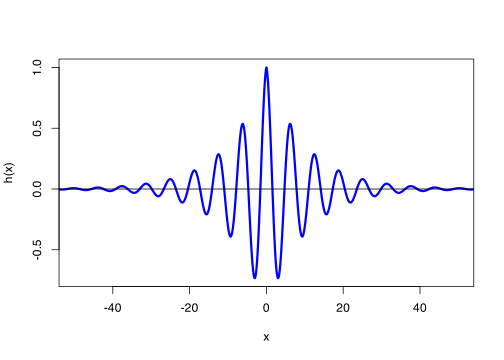
\includegraphics[keepaspectratio]{index_files/mediabag/lectures/L02-mc-uses_files/figure-pdf/h-graph-1.pdf}}

This suggests to me that a mean of 0 and a standard deviation of 20
might work quite well, since this will tend to take values in
\([-40,40]\) or so.

We will use R's function \texttt{dnorm()} for the probability density
function of the normal distribution (which saves us from having to
remember what that is).

\begin{Shaded}
\begin{Highlighting}[]
\NormalTok{n }\OtherTok{\textless{}{-}} \FloatTok{1e6}
\NormalTok{integrand }\OtherTok{\textless{}{-}} \ControlFlowTok{function}\NormalTok{(x) }\FunctionTok{exp}\NormalTok{(}\SpecialCharTok{{-}}\FloatTok{0.1} \SpecialCharTok{*} \FunctionTok{abs}\NormalTok{(x)) }\SpecialCharTok{*} \FunctionTok{cos}\NormalTok{(x)}
\NormalTok{pdf       }\OtherTok{\textless{}{-}} \ControlFlowTok{function}\NormalTok{(x) }\FunctionTok{dnorm}\NormalTok{(x, }\DecValTok{0}\NormalTok{, }\DecValTok{20}\NormalTok{)}
\NormalTok{phi       }\OtherTok{\textless{}{-}} \ControlFlowTok{function}\NormalTok{(x) }\FunctionTok{integrand}\NormalTok{(x) }\SpecialCharTok{/} \FunctionTok{pdf}\NormalTok{(x)}

\NormalTok{samples }\OtherTok{\textless{}{-}} \FunctionTok{rnorm}\NormalTok{(n, }\DecValTok{0}\NormalTok{, }\DecValTok{20}\NormalTok{)}
\FunctionTok{mean}\NormalTok{(}\FunctionTok{phi}\NormalTok{(samples))}
\end{Highlighting}
\end{Shaded}

\begin{verbatim}
[1] 0.2189452
\end{verbatim}

\end{example}

\textbf{Next time:} \emph{We will analyse the accuracy of these Monte
Carlo estimates.}

\textbf{Summary:}

\begin{itemize}
\item
  The indicator \(\Ind_A(x)\) function of a set \(A\) is 1 if
  \(x \in A\) or 0 if \(x \notin A\).
\item
  We can estimate a probability \(\mathbb P(X \in A)\) by using the
  Monte Carlo estimate for \(\Exg\Ind_A(X)\).
\item
  We can estimate an integral \(\int h(x) \, \mathrm{d}x\) by using a
  Monte Carlo estimate with \(\phi(x)\,f(x) = h(x)\).
\end{itemize}

\textbf{Read more:}
\href{https://leeds.primo.exlibrisgroup.com/permalink/44LEE_INST/1fj430b/cdi_askewsholts_vlebooks_9781118728031}{Voss,
\emph{An Introduction to Statistical Computing}}, Section 3.1 and
Subsection 3.2.1.

\chapter{Monte Carlo error I: theory}\label{monte-carlo-error-i-theory}

\[\newcommand{\Exg}{\operatorname{\mathbb{E}}} 
\newcommand{\Ex}{\mathbb{E}} 
\newcommand{\Ind}{\mathbb{I}}
\newcommand{\Var}{\operatorname{Var}}
\newcommand{\Cov}{\operatorname{Cov}}
\newcommand{\Corr}{\operatorname{Corr}}
\newcommand{\ee}{\mathrm{e}}\]

\section{Estimation error}\label{estimation-error}

Today we are going to analysing the accuracy of Monte Carlo estimation.
But before talking about Monte Carlo estimation specifically, let's
first remind ourselves of some concepts about error in statistical
estimation more generally. We will use the following definitions.

\begin{definition}[]\protect\hypertarget{def-stats}{}\label{def-stats}

Let \(\widehat\theta\) be an estimator of a parameter \(\theta\). Then
we have the following definitions of the estimator \(\widehat\theta\):

\begin{itemize}
\item
  The \textbf{bias} is
  \(\operatorname{bias}\big(\widehat\theta\big) = \mathbb E\big(\widehat\theta - \theta\big)  = \mathbb E\widehat\theta - \theta\).
\item
  The \textbf{mean-square error} is
  \(\operatorname{MSE}\big(\widehat\theta\big) = \mathbb E \big(\widehat\theta - \theta\big)^2\).
\item
  The \textbf{root-mean-square error} is the square-root of the
  mean-square error,
  \[\operatorname{RMSE}\big(\widehat\theta\big) = \sqrt{\operatorname{MSE}(\widehat\theta)} = \sqrt{\mathbb E (\widehat\theta - \theta)^2} . \]
\end{itemize}

\end{definition}

Usually, the main goal of estimation is to get the mean-square error of
an estimate as small as possible. This is because the MSE measures by
what distance we are missing on average. It can be easier to interpret
what the root-mean-square error means, as the RMSE has the same units as
the parameter being measured: if \(\theta\) and \(\widehat{\theta}\) are
in metres, say, then the MSE is in metres-squared, whereas the RMSE
error is in metres again. If you minimise the MSE you also minimise the
RMSE and vice versa.

It's nice to have an ``unbiased'' estimator -- that is, one with bias 0.
This is because bias measures any systematic error in a particular
direction. However, unbiasedness by itself is not enough for an estimate
to be good -- we need low variance too. (Remember the old joke about the
statistician who misses his first shot ten yards to the left, misses his
second shot ten yards to the right, then claims to have ``hit the target
on average.'')

(Remember also that ``bias'' is simply the word statisticians use for
\(\mathbb E(\widehat\theta - \theta)\); we don't mean ``bias'' in the
derogatory way it is sometimes used in political arguments, for
example.)

You probably also remember the relationship between the mean-square
error, the bias, and the variance:

\begin{theorem}[]\protect\hypertarget{thm-MSE-bias}{}\label{thm-MSE-bias}

~
\(\operatorname{MSE}\big(\widehat\theta\big) = \operatorname{bias}\big(\widehat\theta\big)^2 + \operatorname{Var}\big(\widehat\theta\big)\).

\end{theorem}

\begin{proof}
The MSE is \begin{align}
  \operatorname{MSE}\big(\widehat\theta\big) = \Exg\big(\widehat\theta - \theta\big)^2
    &= \Exg \big(\widehat\theta^2 - 2\theta\widehat\theta + \theta\big)^2 \\
    &= \Exg \widehat\theta^2 - 2\theta \Exg \widehat\theta + \theta^2 ,
\end{align} where we have expanded the brackets and bought the
expectation inside (remembering that \(\theta\) is a constant). Since
the variance can be written as
\(\Var(\widehat\theta) = \Exg\widehat\theta^2 - (\Exg \widehat\theta)^2\),
we can use a cunning trick of both subtracting and adding
\((\Exg \widehat\theta)^2\). This gives \begin{align}
\operatorname{MSE}\big(\widehat\theta\big)
  &= \Exg \widehat\theta^2 - \big(\!\Exg \widehat\theta\big)^2 + \big(\!\Exg \widehat\theta\big)^2 - 2\theta \Exg \widehat\theta + \theta^2 \\
  &= \Var\big(\widehat\theta\big) + \big( (\Exg \widehat\theta)^2 - 2\theta \Exg \widehat\theta + \theta^2 \big) \\
  &= \Var\big(\widehat\theta\big) + \big( \! \Exg \widehat\theta - \theta\big)^2 \\
  &= \Var\big(\widehat\theta\big) + \operatorname{bias}(\widehat\theta)^2 .
\end{align} This proves the result.
\end{proof}

Since the bias contributes to the mean-square error, that's another
reason to like estimator with low -- or preferably zero -- bias. But
again, unbiasedness isn't enough by itself; we want low variance too.
(There are some situations where there's a ``bias--variance tradeoff'',
where allowing some bias reduces the variance and so can reduce the MSE.
It turns out that Monte Carlo is not one of these cases, however.)

\section{Error of Monte Carlo estimator:
theory}\label{error-of-monte-carlo-estimator-theory}

In this lecture, we're going to be looking more carefully at the size of
the errors made by the Monte Carlo estimator
\[ \widehat{\theta}_n^{\mathrm{MC}} = \frac{1}{n} \big(\phi(X_1) + \phi(X_2) + \cdots + \phi(X_n) \big) = \frac{1}{n} \sum_{i=1}^n \phi(X_i) . \]

Our main result is the following.

\begin{theorem}[]\protect\hypertarget{thm-MCerr}{}\label{thm-MCerr}

Let \(X\) be a random variable, \(\phi\) a function, and
\(\theta = \Exg\phi(X)\). Let
\[ \widehat{\theta}_n^{\mathrm{MC}} = \frac{1}{n} \sum_{i=1}^n \phi(X_i) \]
be the Monte Carlo estimator of \(\theta\). Then:

\begin{enumerate}
\def\labelenumi{\arabic{enumi}.}
\item
  \(\widehat{\theta}_n^{\mathrm{MC}}\) is unbiased, in that
  \(\operatorname{bias}\big(\widehat{\theta}_n^{\mathrm{MC}}\big) = 0\).
\item
  The variance of of \(\widehat{\theta}_n^{\mathrm{MC}}\) is
  \({\displaystyle \operatorname{Var}\big(\widehat{\theta}_n^{\mathrm{MC}}\big) = \frac{1}{n} \operatorname{Var}\big(\phi(X)\big)}\).
\item
  The mean-square error of \(\widehat{\theta}_n^{\mathrm{MC}}\) is
  \({\displaystyle \operatorname{MSE}\big(\widehat{\theta}_n^{\mathrm{MC}}\big) = \frac{1}{n} \operatorname{Var}\big(\phi(X)\big)}\).
\item
  The root-mean-square error of \(\widehat{\theta}_n^{\mathrm{MC}}\) is
  \[{\displaystyle \operatorname{RMSE}\big(\widehat{\theta}_n^{\mathrm{MC}}\big) = \sqrt{\frac{1}{n} \operatorname{Var}\big(\phi(X)\big)} = \frac{1}{\sqrt{n}} \, \operatorname{sd}\big(\phi(X)\big)}. \]
\end{enumerate}

\end{theorem}

Before we get to the proof, let's recap some relevant probability.

Let \(Y_1, Y_2, \dots\) be IID random variables with common expectation
\(\mathbb EY_1 = \mu\) and common variance
\(\operatorname{Var}(Y_1) = \sigma^2\). Consider the mean of the first
\(n\) random variables,
\[ \overline{Y}_n = \frac{1}{n} \sum_{i=1}^n Y_i . \] Then the
expectation of \(\overline{Y}_n\) is
\[ \mathbb E \overline{Y}_n = \mathbb E\left(\frac{1}{n}\sum_{i=1}^n Y_i\right) = \frac{1}{n} 
\sum_{i=1}^n \mathbb{E}Y_i = \frac{1}{n}\,n\,\mu = \mu . \] The variance
of \(\overline{Y}_n\) is
\[ \operatorname{Var}\big(  \overline{Y}_n \big)= \operatorname{Var} \left(\frac{1}{n}\sum_{i=1}^n Y_i\right) = \bigg(\frac{1}{n}\bigg)^2 
\sum_{i=1}^n \operatorname{Var}(Y_i) = \frac{1}{n^2}\,n\,\sigma^2 = \frac{\sigma^2}{n} , \]
where, for this one, we used the independence of the random variables.

\begin{proof}
Apply the probability facts from above with \(Y = \phi(X)\). This gives:

\begin{enumerate}
\def\labelenumi{\arabic{enumi}.}
\item
  \(\Ex \widehat{\theta}_n^{\mathrm{MC}} = \Ex \overline Y_n = \Ex Y = \Exg \phi(X)\),
  so
  \(\operatorname{bias}(\widehat{\theta}_n^{\mathrm{MC}}) = \Exg \phi(X) - \Exg \phi(X) = 0\).
\item
  \({\displaystyle \operatorname{Var}\big(\widehat{\theta}_n^{\mathrm{MC}}\big) = \operatorname{Var}\big(\overline Y_n\big) = \frac{1}{n} \operatorname{Var}(Y) = \frac{1}{n} \operatorname{Var}\big(\phi(X)\big)}\).
\item
  Using Theorem~\ref{thm-MSE-bias},
  \[\operatorname{MSE}(\widehat{\theta}_n^{\mathrm{MC}}) = \operatorname{bias}(\widehat{\theta}_n^{\mathrm{MC}})^2 + \operatorname{Var}(\widehat{\theta}_n^{\mathrm{MC}}) = 0^2 + \frac{1}{n} \operatorname{Var}\big(\phi(X)\big) = \frac{1}{n} \operatorname{Var}\big(\phi(X)\big) . \]
\item
  Take the square root of part 3.
\end{enumerate}

\end{proof}

Let's think about MSE \(\frac{1}{n} \Var(\phi(X))\). The variance terms
is some fixed fact about the random variable \(X\) and the function
\(\phi\). So as \(n\) gets bigger, \(\frac{1}{n}\) gets smaller, so the
MSE gets smaller, and the estimator gets more accurate. This goes back
to what we said when we introduced the Monte Carlo estimator: we get a
more accurate estimate by increasing \(n\). More specifically, the MSE
scales like \(1\n\), or -- perhaps a more useful result -- the RMSE
scales like \(1/\sqrt{n}\). We'll come back to this in the next lecture.

\section{Error of Monte Carlo estimator:
practice}\label{error-of-monte-carlo-estimator-practice}

So when we form a Monte Carlo estimate \(\hat\theta_n^{\text{MC}}\), we
now know it will be unbiased. We'd also like to know it's mean-square
and/or root-mean-square error too.

There's a problem here, though. The reason we are doing Monte Carlo
estimation in the first place is that we \emph{couldn't} calculate
\(\Exg \phi(X)\). So it seems very unlikely we'll be able to calculate
the variance \(\operatorname{Var}(\phi(X))\) either. So how will be able
to assess the mean-square (or root-mean-square) error of our Monte Carlo
estimator?

Well, we can't know it exactly. But we \emph{can} estimate the variance
from the samples we are already using: by taking the sample variance of
the samples \(\phi(x_i)\). That is, we can estimate the variance of the
Monte Carlo estimator by the sample variance
\[ S^2 = \frac{1}{n-1} \sum_{i=1}^n \big(\phi(X_i) - \widehat{\theta}_n^{\mathrm{MC}} \big)^2 . \]
Then we can similarly estimate the mean-square and root-mean-square
errors by
\[ \text{MSE} \approx \frac{1}{n}S^2 \qquad \text{and} \qquad \text{RMSE} \approx \sqrt{\frac{1}{n} S^2} = \frac{1}{\sqrt{n}}\,S  \]
respectively.

\begin{example}[]\protect\hypertarget{exm-MCexp2}{}\label{exm-MCexp2}

Let's go back to the very first example in the module,
Example~\ref{exm-MCexp}, where we were trying to find the expectation of
an \(\operatorname{Exp}(2)\) random variable. We used this R code:

\begin{Shaded}
\begin{Highlighting}[]
\NormalTok{n }\OtherTok{\textless{}{-}} \FloatTok{1e6}
\NormalTok{samples }\OtherTok{\textless{}{-}} \FunctionTok{rexp}\NormalTok{(n, }\DecValTok{2}\NormalTok{)}
\NormalTok{MCest }\OtherTok{\textless{}{-}} \FunctionTok{mean}\NormalTok{(samples)}
\NormalTok{MCest}
\end{Highlighting}
\end{Shaded}

\begin{verbatim}
[1] 0.5006352
\end{verbatim}

(Because Monte Carlo estimation is random, this won't be the
\emph{exact} same estimate we had before, of course.)

So if we want to investigate the error, we can use the sample variance
of these samples. We will use the sample variance function
\texttt{var()} to calculate the sample variance. In this simple case,
the function is \(\phi(x) = x\), so we need only use the variance of the
samples themselves.

\begin{Shaded}
\begin{Highlighting}[]
\NormalTok{var\_est }\OtherTok{\textless{}{-}} \FunctionTok{var}\NormalTok{(samples)}
\NormalTok{MSEest  }\OtherTok{\textless{}{-}}\NormalTok{ var\_est }\SpecialCharTok{/}\NormalTok{ n}
\NormalTok{RMSEest }\OtherTok{\textless{}{-}} \FunctionTok{sqrt}\NormalTok{(MSEest)}
\FunctionTok{c}\NormalTok{(var\_est, MSEest, RMSEest)}
\end{Highlighting}
\end{Shaded}

\begin{verbatim}
[1] 2.503570e-01 2.503570e-07 5.003569e-04
\end{verbatim}

The first number is \texttt{var\_est} \(= 0.25\), the sample variance of
our \(\phi(x_i)\)s:\\
\[ s^2 = \frac{1}{n-1} \sum_{i=1}^n \big(\phi(x_i) - \widehat{\theta}_n^{\mathrm{MC}}\big)^2 . \]
This should be a good estimate of the true variance
\(\operatorname{Var}(\phi(X))\). In fact, in this simple case, we know
that \(\operatorname{Var}(X) = \frac{1}{2^2} = 0.25\), so we know that
the estimate was good. In calculating this in the code, we used R's
\texttt{var()} function, which calculates the sample variance of some
values.

The second number is \texttt{MSEest}
\(= \ensuremath{2.504\times 10^{-7}}\), our estimate of the mean-square
error. Since
\(\operatorname{MSE}(\widehat{\theta}_n^{\mathrm{MC}}) = \frac{1}{n} \operatorname{Var}(\phi(X))\),
then \(\frac{1}{n} s^2\) should be a good estimate of the MSE.

The third number is \texttt{RMSEest} \(= \ensuremath{5\times 10^{-4}}\)
our estimate of the root-mean square error, which is simply the
square-root of our estimate of the mean-square error.

\end{example}

\begin{example}[]\protect\hypertarget{exm-MCexp2}{}\label{exm-MCexp2}

In Example~\ref{exm-MCprob}, we were estimating \(\mathbb P(Z > 2)\),
where \(Z\) is a standard normal.

Our code was

\begin{Shaded}
\begin{Highlighting}[]
\NormalTok{n }\OtherTok{\textless{}{-}} \FloatTok{1e6}
\NormalTok{samples }\OtherTok{\textless{}{-}} \FunctionTok{rnorm}\NormalTok{(n)}
\NormalTok{MCest }\OtherTok{\textless{}{-}} \FunctionTok{mean}\NormalTok{(samples }\SpecialCharTok{\textgreater{}} \DecValTok{2}\NormalTok{)}
\NormalTok{MCest}
\end{Highlighting}
\end{Shaded}

\begin{verbatim}
[1] 0.022458
\end{verbatim}

So our root-mean-square error can be approximated as

\begin{Shaded}
\begin{Highlighting}[]
\NormalTok{MSEest }\OtherTok{\textless{}{-}} \FunctionTok{var}\NormalTok{(samples }\SpecialCharTok{\textgreater{}} \DecValTok{2}\NormalTok{) }\SpecialCharTok{/}\NormalTok{ n}
\FunctionTok{sqrt}\NormalTok{(MSEest)}
\end{Highlighting}
\end{Shaded}

\begin{verbatim}
[1] 0.0001481677
\end{verbatim}

since \texttt{samples\ \textgreater{}\ 2} is the indicator function of
whether \(X_i > 2\) or not.

\end{example}

\textbf{Next time:} \emph{We'll continue analysing Monte Carlo error,
looking at confidence intervals and assessing how many samples to
take..}

\textbf{Summary:}

\begin{itemize}
\item
  The Monte Carlo estimator is unbiased.
\item
  The Monte Carlo estimator has mean-square error \(\Var(\phi(X))/n\),
  so the root-mean-square error scales like \(1/\sqrt{n}\).
\item
  The mean-square error can be estimated by \(S^2 / n\), where \(S^2\)
  is the sample variance of the \(\phi(X_i)\).
\end{itemize}

\textbf{Read more:}
\href{https://leeds.primo.exlibrisgroup.com/permalink/44LEE_INST/1fj430b/cdi_askewsholts_vlebooks_9781118728031}{Voss,
\emph{An Introduction to Statistical Computing}}, Subsection 3.2.2.

\chapter*{Problem Sheet 1}\label{P1}
\addcontentsline{toc}{chapter}{Problem Sheet 1}

\markboth{Problem Sheet 1}{Problem Sheet 1}

This is Problem Sheet 1, which covers material from Lectures 1 to 6. You
should work through all the questions on this problem sheet in advance
of the problems class, which takes place in the lecture of
\textbf{Thursday 16 October}. If you are stuck on any of the questions,
you are welcome to discuss them with me in my office hours on Thursdays
at 1300.

This problem sheet is to help you practice material from the module and
to help you check your learning. It is \emph{not} for formal assessment
and does not count towards your module mark.

However, if, optionally, you would like some brief informal feedback on
\textbf{Questions 4, 6 and 8} (marked ★), I am happy to provide some. If
you want some brief feedback, you should submit your work electronically
through Gradescope via the module's Minerva page by \textbf{1400 on
Tuesday 14 October}. I will return some brief comments on your those two
questions by the problems class on Thursday 16 October. Because this
informal feedback, not part of the official assessment, I cannot accept
late work for any reason -- but I am always happy to discuss any of your
work on any question in my office hours.

Many of these questions will require use of the
\href{https://cran.r-project.org}{R programming language} (for example,
by using the \href{https://posit.co/downloads/}{program RStudio}).

Full solutions should be released on Friday 17 October.

\[\newcommand{\Exg}{\operatorname{\mathbb{E}}} 
\newcommand{\Ex}{\mathbb{E}} 
\newcommand{\Ind}{\mathbb{I}}
\newcommand{\Var}{\operatorname{Var}}
\newcommand{\Cov}{\operatorname{Cov}}
\newcommand{\Corr}{\operatorname{Corr}}
\newcommand{\ee}{\mathrm{e}}\]

\textbf{1.} ~~~~~Let \(X\) be uniform on \([-1,2]\).

\textbf{(a)} ~~By hand, calculate the exact value of \(\Ex X^4\).

\emph{Solution.}

\[\int_{-1}^2 x^4\,\frac{1}{2-(-1)}\,\mathrm{d}x = \tfrac13 \Big[\tfrac15x^5\Big]_{-1}^2 = \tfrac13\Big(\tfrac{32}{5}-\big(-\tfrac15\big)\Big) = \tfrac{33}{15} = \tfrac{11}{5} = 2.2\]

\textbf{(b)} ~~Using R, calculate a Monte Carlo estimate for
\(\Ex X^4\).

\emph{Solution.} I used the R code

\begin{Shaded}
\begin{Highlighting}[]
\NormalTok{n }\OtherTok{\textless{}{-}} \FloatTok{1e6}
\NormalTok{samples }\OtherTok{\textless{}{-}} \FunctionTok{runif}\NormalTok{(n, }\SpecialCharTok{{-}}\DecValTok{1}\NormalTok{, }\DecValTok{2}\NormalTok{)}
\FunctionTok{mean}\NormalTok{(samples}\SpecialCharTok{\^{}}\DecValTok{4}\NormalTok{)}
\end{Highlighting}
\end{Shaded}

\begin{verbatim}
[1] 2.200851
\end{verbatim}

\textbf{2.} ~~~~~Let \(X\) and \(Y\) both be standard normal
distributions. Compute a Monte Carlo estimate of \(\Exg \max\{X,Y\}\).
(You may wish to investigate R's \texttt{pmax()} function.)

\emph{Solution.} By looking at \texttt{?pmax} (or maybe searching on
Google) I discovered that \texttt{pmax()} gives the ``parallel maxima''
of two (or more vectors). That is the first element is the maximum of
all the first elements of the vectors; the second element is the maximum
of all the second elements of the vectors; and so on.

So I used the R code

\begin{Shaded}
\begin{Highlighting}[]
\NormalTok{n }\OtherTok{\textless{}{-}} \FloatTok{1e6}
\NormalTok{xsamples }\OtherTok{\textless{}{-}} \FunctionTok{rnorm}\NormalTok{(n)}
\NormalTok{ysamples }\OtherTok{\textless{}{-}} \FunctionTok{rnorm}\NormalTok{(n)}
\FunctionTok{mean}\NormalTok{(}\FunctionTok{pmax}\NormalTok{(xsamples, ysamples))}
\end{Highlighting}
\end{Shaded}

\begin{verbatim}
[1] 0.5649173
\end{verbatim}

\textbf{3.} ~~~~~You are trapped alone on an island. All you have with
you is a tin can (radius \(r\)) and a cardboard box (side lengths
\(2r \times 2r\)) that it fits snugly inside. You put the can inside the
box {[}left picture{]}.

When it starts raining, each raindrop that falls in the cardboard box
might fall into the tin can {[}middle picture{]}, or might fall into the
corners of the box outside the can {[}right picture{]}.


\includegraphics[width=6.25in,height=\textheight,keepaspectratio]{index_files/mediabag/problems/P1-can-box.pdf}

\textbf{(a)} ~~Using R, simulate rainfall into the box. You may take
units such that \(r = 1\). Estimate the probability \(\theta\) that a
uniformly-random raindrop that falls in the cardboard box falls into the
tin can also.

\emph{Solution.} I set things up so that the box is \([-1, 1]^2\),
centered at the origin. This means that the inside of the can is the set
of points is those \((x,y)\) such that \(x^2 + y^2 \leq 1\).

\begin{Shaded}
\begin{Highlighting}[]
\NormalTok{n }\OtherTok{\textless{}{-}} \FloatTok{1e6}
\NormalTok{rain\_x }\OtherTok{\textless{}{-}} \FunctionTok{runif}\NormalTok{(n, }\SpecialCharTok{{-}}\DecValTok{1}\NormalTok{, }\DecValTok{1}\NormalTok{)}
\NormalTok{rain\_y }\OtherTok{\textless{}{-}} \FunctionTok{runif}\NormalTok{(n, }\SpecialCharTok{{-}}\DecValTok{1}\NormalTok{, }\DecValTok{1}\NormalTok{)}
\NormalTok{in\_box }\OtherTok{\textless{}{-}} \ControlFlowTok{function}\NormalTok{(x, y) x}\SpecialCharTok{\^{}}\DecValTok{2} \SpecialCharTok{+}\NormalTok{ y}\SpecialCharTok{\^{}}\DecValTok{2} \SpecialCharTok{\textless{}=} \DecValTok{1}
\FunctionTok{mean}\NormalTok{(}\FunctionTok{in\_box}\NormalTok{(rain\_x, rain\_y))}
\end{Highlighting}
\end{Shaded}

\begin{verbatim}
[1] 0.785571
\end{verbatim}

\textbf{(b)} ~~Calculate exactly the probability \(\theta\).

\emph{Solution.} The area of the box is \(2r \times 2r = 4r^2\). The
area of the can is \(\pi r^2\). So the probability a raindrop landing in
the box lands in the can is
\[ \frac{\text{area of can}}{\text{area of box}} = \frac{\pi r^2}{4r^2} = \frac{\pi}{4} \approx 0.785. \]

\textbf{(c)} ~~You realise that, despite being trapped all alone on the
island, you now have a way of approximating the value of \(\pi\). If you
want to calculate \(\pi\) to 6 decimal places, roughly how many
raindrops do you need to fall into the box?

\emph{Solution.} The phrase ``to 6 decimal places'' isn't a precise
mathematical one. I'm going to interpret this as getting the
root-mean-square error below \(10^{-6}\). If you interpret it slightly
differently that's fine -- for example, getting the width of a 95\%
confidence interval below \(10^{-6}\) could be another, slightly
stricter, criterion.

One could work this out by hand. Since the variance of a Bernoulli
random variable is \(p(1-p)\), the mean-square error of our estimator is
\[ \frac{\frac{\pi}{4}(1 - \frac{\pi}{4})}{n} \approx \frac{0.169}{n} . \]
So we need
\[n = \frac{0.169}{(10^{-6})^2} \approx 169 \text{ billion} . \]

That said, if we are trapped on our desert island, maybe we don't know
what \(\frac{\pi}{4}(1 - \frac{\pi}{4})\) is. In that case we could do
this using the can and the box. Our estimate of the variance is

\begin{Shaded}
\begin{Highlighting}[]
\NormalTok{var\_est }\OtherTok{\textless{}{-}} \FunctionTok{var}\NormalTok{(}\FunctionTok{in\_box}\NormalTok{(rain\_x, rain\_y))}
\NormalTok{var\_est }\SpecialCharTok{/}\NormalTok{ (}\FloatTok{1e{-}6}\NormalTok{)}\SpecialCharTok{\^{}}\DecValTok{2}
\end{Highlighting}
\end{Shaded}

\begin{verbatim}
[1] 168449372405
\end{verbatim}

We will probably spend a long time waiting for that much rain!

\textbf{4.}~~~~~★ \emph{(2024--25 exam, Question 1(d))} A statistician
wants to estimate \(\mathbb E(\cos X)\), where
\(X \sim \operatorname{Exp(4)}\) is an exponential distribution with
rate 4. The statistician begins with a pilot study, as shown in the R
session below:

\begin{Shaded}
\begin{Highlighting}[]
   \SpecialCharTok{\textgreater{}}\NormalTok{ n }\OtherTok{\textless{}{-}} \FloatTok{1e4}
\SpecialCharTok{\textgreater{}}\NormalTok{ samples }\OtherTok{\textless{}{-}} \FunctionTok{rexp}\NormalTok{(n, }\DecValTok{4}\NormalTok{)}
\SpecialCharTok{\textgreater{}} \FunctionTok{var}\NormalTok{(}\FunctionTok{cos}\NormalTok{(samples))}
\NormalTok{[}\DecValTok{1}\NormalTok{] }\FloatTok{0.01416}
\end{Highlighting}
\end{Shaded}

~~~~~~~~~~~~The statistician wants to get the root-mean-square error of
her estimator down to \(10^{−4}\). Approximately how many samples will
she need for the full study? Explain your answer.

\textbf{5.} ~~~~~Let \(h(x) = 1/(x + 0.1)\). We wish to estimate
\(\int_0^5 h(x) \, \mathrm{d}x\) using a Monte Carlo method.

\textbf{(a)} ~~Estimate the integral using \(X\) uniform on \([0,5]\).

\emph{Solution.}

\begin{Shaded}
\begin{Highlighting}[]
\NormalTok{n }\OtherTok{\textless{}{-}} \FloatTok{1e6}
\NormalTok{integrand }\OtherTok{\textless{}{-}} \ControlFlowTok{function}\NormalTok{(x) }\DecValTok{1} \SpecialCharTok{/}\NormalTok{ (x }\SpecialCharTok{+} \FloatTok{0.1}\NormalTok{)}
\NormalTok{samples1 }\OtherTok{\textless{}{-}} \FunctionTok{runif}\NormalTok{(n, }\DecValTok{0}\NormalTok{, }\DecValTok{5}\NormalTok{)}
\FunctionTok{mean}\NormalTok{(}\DecValTok{5} \SpecialCharTok{*} \FunctionTok{integrand}\NormalTok{(samples1))}
\end{Highlighting}
\end{Shaded}

\begin{verbatim}
[1] 3.939012
\end{verbatim}

(In fact, the true answer is \(\log(5.1) - \log(0.1) = 3.932\), so it
looks like this is working correctly.)

\textbf{(b)} ~~Can you come up with a choice of \(X\) that improves on
the estimate from (a)?

\emph{Solution.} Let's look at a graph of the integrand \(h\).

\begin{Shaded}
\begin{Highlighting}[]
\FunctionTok{curve}\NormalTok{(}
\NormalTok{  integrand, }\AttributeTok{n =} \DecValTok{1001}\NormalTok{, }\AttributeTok{from =} \DecValTok{0}\NormalTok{, }\AttributeTok{to =} \DecValTok{5}\NormalTok{,}
  \AttributeTok{col =} \StringTok{"blue"}\NormalTok{, }\AttributeTok{lwd =} \DecValTok{3}\NormalTok{,}
  \AttributeTok{xlab =} \StringTok{"x"}\NormalTok{, }\AttributeTok{ylab =} \StringTok{"integrand h(x)"}\NormalTok{, }\AttributeTok{xlim =} \FunctionTok{c}\NormalTok{(}\DecValTok{0}\NormalTok{,}\DecValTok{5}\NormalTok{)}
\NormalTok{)}
\FunctionTok{abline}\NormalTok{(}\AttributeTok{h =} \DecValTok{0}\NormalTok{)}
\end{Highlighting}
\end{Shaded}

\pandocbounded{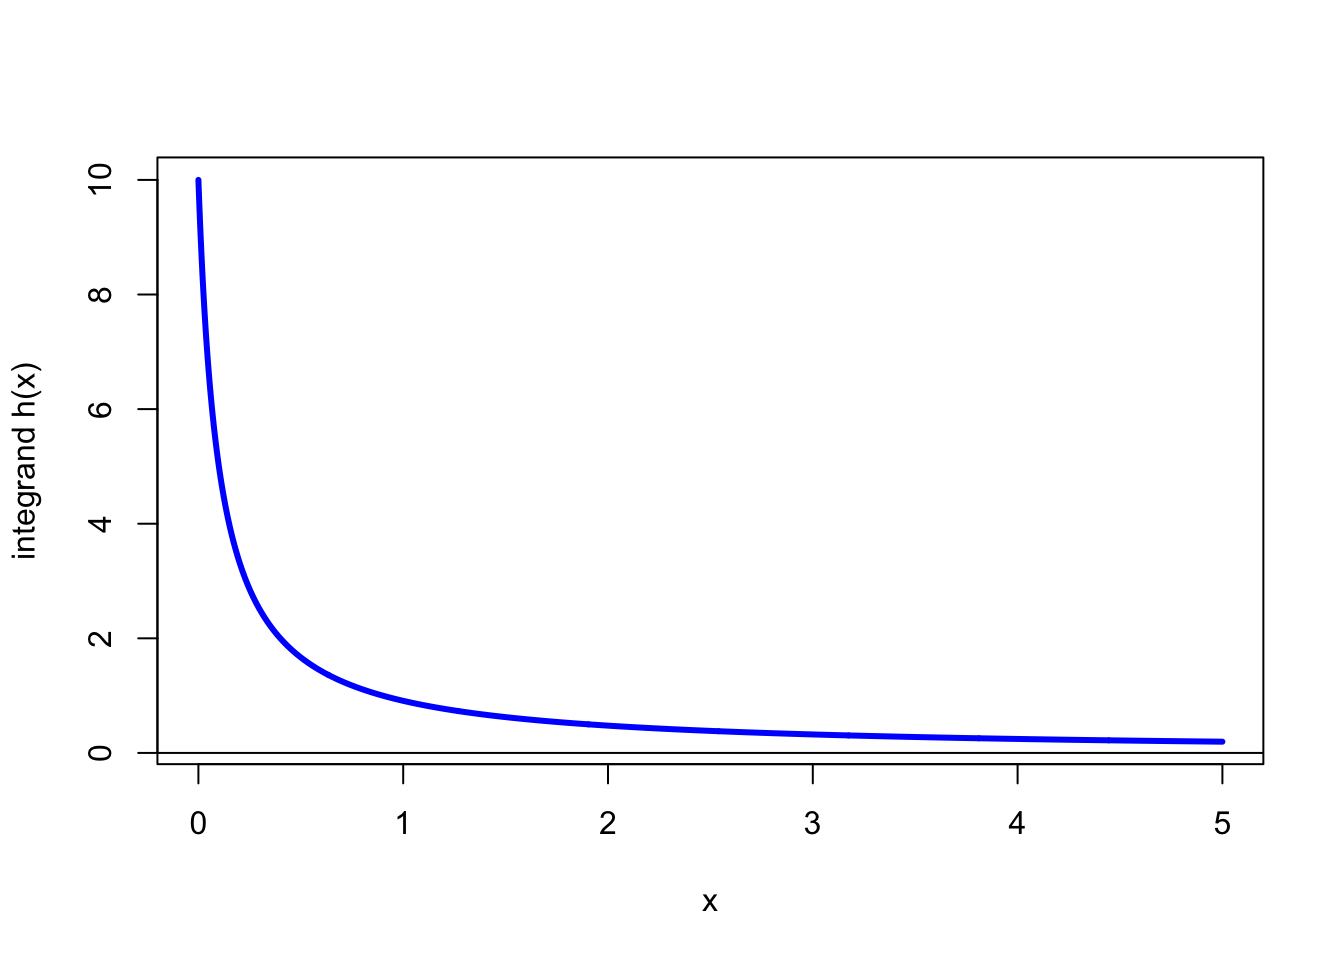
\includegraphics[keepaspectratio]{index_files/mediabag/problems/P1_files/figure-pdf/h2-graph-1.pdf}}

We see that we get a much bigger contribution to the integral from
values near 0. So a random variable that picks values nearer to 0 more
often might have a chance of giving a more accurate result.

I decided to try an exponential distribution with rate 1, which should
sample the smaller values of \(x\) more often.

\begin{Shaded}
\begin{Highlighting}[]
\NormalTok{pdf }\OtherTok{\textless{}{-}} \ControlFlowTok{function}\NormalTok{(x) }\FunctionTok{dexp}\NormalTok{(x, }\DecValTok{1}\NormalTok{)}
\NormalTok{phi }\OtherTok{\textless{}{-}} \ControlFlowTok{function}\NormalTok{(x) (}\FunctionTok{integrand}\NormalTok{(x) }\SpecialCharTok{/} \FunctionTok{pdf}\NormalTok{(x)) }\SpecialCharTok{*}\NormalTok{ (x }\SpecialCharTok{\textless{}=} \DecValTok{5}\NormalTok{)}

\NormalTok{samples2 }\OtherTok{\textless{}{-}} \FunctionTok{rexp}\NormalTok{(n, }\DecValTok{1}\NormalTok{)}
\FunctionTok{mean}\NormalTok{(}\FunctionTok{phi}\NormalTok{(samples2))}
\end{Highlighting}
\end{Shaded}

\begin{verbatim}
[1] 3.934066
\end{verbatim}

(I had to include \texttt{x\ \textless{}=\ 5} in the expression for
\(\phi\), because my exponential distribution will sometimes take
samples above 5, but they should count as 0 in an estimate for the
integral between 0 and 5.)

To see whether or not this was an improvement, I estimated the
mean-square error.

\begin{Shaded}
\begin{Highlighting}[]
\FunctionTok{var}\NormalTok{(}\DecValTok{5} \SpecialCharTok{*} \FunctionTok{integrand}\NormalTok{(samples1)) }\SpecialCharTok{/}\NormalTok{ n}
\end{Highlighting}
\end{Shaded}

\begin{verbatim}
[1] 3.369629e-05
\end{verbatim}

\begin{Shaded}
\begin{Highlighting}[]
\FunctionTok{var}\NormalTok{(}\FunctionTok{phi}\NormalTok{(samples2)) }\SpecialCharTok{/}\NormalTok{ n}
\end{Highlighting}
\end{Shaded}

\begin{verbatim}
[1] 6.092281e-06
\end{verbatim}

I found that I had reduced the mean-square error by roughly a factor of
5.

\textbf{6.} ~~~~~★ Show that the indicator functions \(\mathbb I_A(X)\)
and \(\mathbb I_B(X)\) have correlation 0 if and only if the events
\(\{X \in A\}\) and \(\{X \in B\}\) are independent.

\emph{Solution.} Recall that two random variables \(U\), \(V\) have
correlation 0 if and only if their covariance
\(\Cov(U,V) = \Ex UV - (\Ex U)(\Ex V)\) is 0 too.

We know that \(\Exg\Ind_A(X) = \mathbb P(X \in A)\) and
\(\Exg \Ind_B(Y) = \mathbb P(X \in B)\). What about
\(\Exg \Ind_A(X) \Ind_B(X)\)? Well, \(\Ind_A(x) \Ind_B(x)\) is 1 if and
only if \emph{both} indicator functions equal 1, which is if and only if
both \(x \in A\) and \(x \in B\). So
\(\Exg \Ind_A(X) \Ind_B(X) = \mathbb P(X \in A \text{ and } X \in B)\).

So the covariance is
\[ \Cov \big(\Ind_A(X), \Ind_B(X) \big) = \mathbb P(X \in A \text{ and } X \in B) - \mathbb P(X \in A)\, \mathbb P(X \in B) . \]
If this is 0, then
\(\mathbb P(X \in A \text{ and } X \in B) = \mathbb P(X \in A)\, \mathbb P(X \in B)\),
which is precisely the definition of those two events being independent.

\textbf{7.} ~~~~~Let \(X\) be an exponential distribution with rate 1.

\textbf{(a)} ~~Estimate \(\mathbb EX^{2.1}\) using the standard Monte
Carlo method.

\begin{Shaded}
\begin{Highlighting}[]
\NormalTok{n }\OtherTok{\textless{}{-}} \FloatTok{1e6}
\NormalTok{samples }\OtherTok{\textless{}{-}} \FunctionTok{rexp}\NormalTok{(n, }\DecValTok{1}\NormalTok{)}
\FunctionTok{mean}\NormalTok{(samples}\SpecialCharTok{\^{}}\FloatTok{2.1}\NormalTok{)}
\end{Highlighting}
\end{Shaded}

\begin{verbatim}
[1] 2.195702
\end{verbatim}

\textbf{(b)} ~~Estimate \(\mathbb EX^{2.1}\) using \(X^2\) as a control
variate. (You may recall that if \(Y\) is exponential with rate
\(\lambda\) then \(\mathbb EY^2 = 2/\lambda^2\).)

\emph{Solution.} We have \(\Ex X^2 = 2\). So, re-using the same sample
as before (you don't have to do this -- you could take new samples), our
R code is as follows.

\begin{Shaded}
\begin{Highlighting}[]
\FunctionTok{mean}\NormalTok{(samples}\SpecialCharTok{\^{}}\FloatTok{2.1} \SpecialCharTok{{-}}\NormalTok{ samples}\SpecialCharTok{\^{}}\DecValTok{2}\NormalTok{) }\SpecialCharTok{+} \DecValTok{2}
\end{Highlighting}
\end{Shaded}

\begin{verbatim}
[1] 2.197517
\end{verbatim}

\textbf{(c)} ~~Which method is better?

\emph{Solution.} The better answer is the one with the smaller
mean-square error.

For the basic method,

\begin{Shaded}
\begin{Highlighting}[]
\FunctionTok{var}\NormalTok{(samples}\SpecialCharTok{\^{}}\FloatTok{2.1}\NormalTok{) }\SpecialCharTok{/}\NormalTok{ n}
\end{Highlighting}
\end{Shaded}

\begin{verbatim}
[1] 2.799048e-05
\end{verbatim}

For the control variate method,

\begin{Shaded}
\begin{Highlighting}[]
\FunctionTok{var}\NormalTok{(samples}\SpecialCharTok{\^{}}\FloatTok{2.1} \SpecialCharTok{{-}}\NormalTok{ samples}\SpecialCharTok{\^{}}\DecValTok{2}\NormalTok{) }\SpecialCharTok{/}\NormalTok{ n}
\end{Highlighting}
\end{Shaded}

\begin{verbatim}
[1] 6.884677e-07
\end{verbatim}

So the control variates method is much, much better.

\textbf{8.} ~~~~~★ Let \(Z\) be a standard normal distribution. A
statistician has been investigating Monte Carlo estimates of
\(\mathbb EZ^k\) for different positive integers values of \(k\). Her
colleague suggests using \(Z' = -Z\) as an antithetic variable. Without
running any R code, explain whether or not this is a good idea
\textbf{(a)} when \(k\) is even; \textbf{(b)} when \(k\) is odd.

\emph{Solution.}

\textbf{(a)} When \(k\) is even, we have \(Z^k = (-Z)^k\). So the
antithetic variables method just repeats each sample twice. This is
obviously no benefit at all, and just wastes time. Indeed, we have
perfect positive correlation \(\rho = +1\), which is the ``worst-case
scenario''.

\textbf{(b)} When \(k\) is odd, we have \(Z^k = -(-Z)^k\). In this case
we know that \(\Ex Z^k = 0\), because the results for positive \(z\)
exactly balance out those for negative \(z\), so no Monte Carlo sampling
is necessary. If our statistician has somehow forgotten that, though,
she will get a pleasant surprise! After just two samples, she will get
the estimate
\[\frac{1}{2} \big(Z_1^k + (-Z_1)^k \big) = \frac{1}{2} (Z_1^k - Z_1^k) = 0 ,\]
Thereby getting the result exactly right. Indeed, we have perfect
negative correlation \(\rho = -1\), which is the ``best-case scenario''.




\end{document}
